\documentclass[10pt]{beamer}\usepackage[]{graphicx}\usepackage[]{color}
%% maxwidth is the original width if it is less than linewidth
%% otherwise use linewidth (to make sure the graphics do not exceed the margin)
\makeatletter
\def\maxwidth{ %
  \ifdim\Gin@nat@width>\linewidth
    \linewidth
  \else
    \Gin@nat@width
  \fi
}
\makeatother

\definecolor{fgcolor}{rgb}{0.345, 0.345, 0.345}
\newcommand{\hlnum}[1]{\textcolor[rgb]{0.686,0.059,0.569}{#1}}%
\newcommand{\hlstr}[1]{\textcolor[rgb]{0.192,0.494,0.8}{#1}}%
\newcommand{\hlcom}[1]{\textcolor[rgb]{0.678,0.584,0.686}{\textit{#1}}}%
\newcommand{\hlopt}[1]{\textcolor[rgb]{0,0,0}{#1}}%
\newcommand{\hlstd}[1]{\textcolor[rgb]{0.345,0.345,0.345}{#1}}%
\newcommand{\hlkwa}[1]{\textcolor[rgb]{0.161,0.373,0.58}{\textbf{#1}}}%
\newcommand{\hlkwb}[1]{\textcolor[rgb]{0.69,0.353,0.396}{#1}}%
\newcommand{\hlkwc}[1]{\textcolor[rgb]{0.333,0.667,0.333}{#1}}%
\newcommand{\hlkwd}[1]{\textcolor[rgb]{0.737,0.353,0.396}{\textbf{#1}}}%
\let\hlipl\hlkwb

\usepackage{framed}
\makeatletter
\newenvironment{kframe}{%
 \def\at@end@of@kframe{}%
 \ifinner\ifhmode%
  \def\at@end@of@kframe{\end{minipage}}%
  \begin{minipage}{\columnwidth}%
 \fi\fi%
 \def\FrameCommand##1{\hskip\@totalleftmargin \hskip-\fboxsep
 \colorbox{shadecolor}{##1}\hskip-\fboxsep
     % There is no \\@totalrightmargin, so:
     \hskip-\linewidth \hskip-\@totalleftmargin \hskip\columnwidth}%
 \MakeFramed {\advance\hsize-\width
   \@totalleftmargin\z@ \linewidth\hsize
   \@setminipage}}%
 {\par\unskip\endMakeFramed%
 \at@end@of@kframe}
\makeatother

\definecolor{shadecolor}{rgb}{.97, .97, .97}
\definecolor{messagecolor}{rgb}{0, 0, 0}
\definecolor{warningcolor}{rgb}{1, 0, 1}
\definecolor{errorcolor}{rgb}{1, 0, 0}
\newenvironment{knitrout}{}{} % an empty environment to be redefined in TeX

\usepackage{alltt}%
\usetheme{Boadilla}
\usecolortheme{seahorse}

\usepackage[utf8]{inputenc}%


\usepackage[normalem]{ulem}%strikeout
 

% graphics
%% Figures %%%%%%%%%%%%%%%%%%%%%%%%%%%%%%%%%%%%%%%%%%%%%%%%%%
\usepackage{graphicx}
\usepackage{xcolor}%for color mixing

\usepackage{amsmath}%
\usepackage{amsfonts}%
\usepackage{amssymb}%
\usepackage{graphicx}

\usepackage{tikz}

%%%%%%%%%%%%%%%%%%%%%%%%%%%%%%%%%%%%%%%%%%%%%%
%%%%%%%%%%%%%%%%% Doc info %%%%%%%%%%%%%%%%%%%
\title[\textbf{Linear models 3:}]{Multiple regressions and interactions}
\date{\today}

%%%%%%%%%%%%%%%%%%%%%%%%%%%%%%%%%%%%
\IfFileExists{upquote.sty}{\usepackage{upquote}}{}
\begin{document}




\begin{frame}
\maketitle	
\end{frame}
%%%%%%%%%%%

\AtBeginSection[]
{
  \begin{frame}<beamer>
    \frametitle{}
    \tableofcontents[currentsection,hideothersubsections,subsectionstyle=hide]% down vote\tableofcontents[currentsection,currentsubsection,hideothersubsections,sectionstyle=show/hide,subsectionstyle=show/shaded/hide] 
  \end{frame}
} 



%%%%%%%%%%%%%%%%%%%%%%%%%%%%%%%%%%%%%%%%%%%%%%%%%%%%%%%%%%%%%%%%%%%
%%%%%%%%%%%%%%%%%%%%%%%%%%%%%%%%%%%%%%%%%%%%%%%%%%%%%%%%%%%%%%%%%%%
\section{Linear model, reminder}

\begin{frame}[fragile]{A simple linear model}
  \textbf{{\color{purple}{Response}} = {\color{blue}{Intercept}} + {\color{red}{Slope}} $\times$ {\color{orange}{Predictor}} + {\color{gray}{Error}}} \\
  
\begin{knitrout}\small
\definecolor{shadecolor}{rgb}{0.843, 0.867, 0.922}\color{fgcolor}
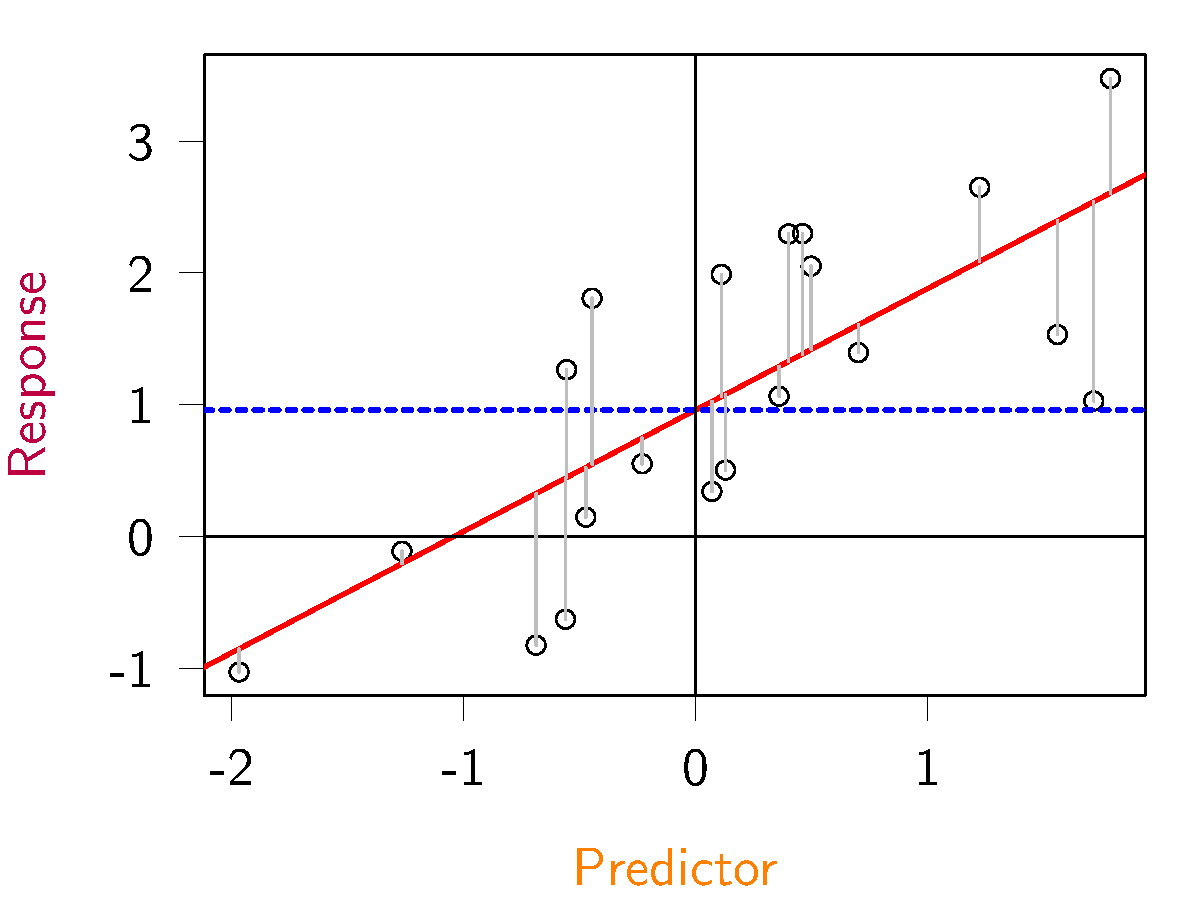
\includegraphics[width=0.8\textwidth,height=0.6\textwidth]{figure/lmprinc-1} 

\end{knitrout}
\end{frame}
%%%%%%%%%%%

\begin{frame}[fragile]{A simple linear model}
  \textbf{{\color{purple}{Response}} = {\color{blue}{Intercept}} + {\color{red}{Slope1}} $\times$ {\color{orange}{Predictor1}} + {\color{red}{Slope2}} $\times$ {\color{orange}{Predictor2}}  + {\color{gray}{Error}}} \\
  \vspace{1cm}
\textbf{In R:}
\begin{knitrout}\small
\definecolor{shadecolor}{rgb}{0.843, 0.867, 0.922}\color{fgcolor}\begin{kframe}
\begin{alltt}
  \hlkwd{lm}\hlstd{(response} \hlopt{~} \hlnum{1} \hlopt{+} \hlstd{predictor1} \hlopt{+} \hlstd{predictor2,} \hlkwc{data}\hlstd{=data)}
\end{alltt}
\end{kframe}
\end{knitrout}


\end{frame}
%%%%%%%%%%%

%%%%%%%%%%%%%%%%%%%%%%%%%%%%%%%%%%%%%%%%%%%%%%%%%%%%%%%%%%%%%%%%%%%%%%%%%%%%%%%%%%%%%%%%%%%%%%%%%%%%
\section{Multiple regression}


\section{Interaction}

\begin{frame}[fragile]{Warnings}

  \begin{alertblock}{Vocabulary warning!}
    \begin{itemize}[<+->]
      \item \textit{correlation}: linear association between two variables "how well does $x$ explain $y$ ?"
      \item \textit{interaction}: non-additive effect of two or more variables "does the effect of $x_1$ on $y$ change as a function of $x_2$?"
    \end{itemize}
  \end{alertblock}

\pause 
\begin{knitrout}\small
\definecolor{shadecolor}{rgb}{0.843, 0.867, 0.922}\color{fgcolor}
\includegraphics[width=0.6\textwidth,height=0.6\textheight]{figure/histinter-1} 

\end{knitrout}
\end{frame}
%%%%%%%%%%%

\begin{frame}[fragile]{Fitting an interaction}

    
\begin{knitrout}\small
\definecolor{shadecolor}{rgb}{0.843, 0.867, 0.922}\color{fgcolor}\begin{kframe}
\begin{alltt}
  \hlkwd{lm}\hlstd{(y} \hlopt{~} \hlnum{1} \hlopt{+} \hlstd{x1} \hlopt{*} \hlstd{x2)}
  \hlkwd{lm}\hlstd{(y} \hlopt{~} \hlnum{1} \hlopt{+} \hlstd{x1} \hlopt{+} \hlstd{x2} \hlopt{+} \hlstd{x1}\hlopt{:}\hlstd{x2)}
\end{alltt}
\end{kframe}
\end{knitrout}
  \pause
\begin{knitrout}\small
\definecolor{shadecolor}{rgb}{0.843, 0.867, 0.922}\color{fgcolor}\begin{kframe}
\begin{alltt}
  \hlkwd{summary}\hlstd{(}\hlkwd{lm}\hlstd{(y}\hlopt{~} \hlnum{1} \hlopt{+} \hlstd{x1}\hlopt{*}\hlstd{x2))}
\end{alltt}
\begin{verbatim}

Call:
lm(formula = y ~ 1 + x1 * x2)

Residuals:
    Min      1Q  Median      3Q     Max 
-1.8719 -0.6777 -0.1086  0.5897  2.3166 

Coefficients:
            Estimate Std. Error t value Pr(>|t|)    
(Intercept)  1.14098    0.09578  11.913  < 2e-16 ***
x1          -0.49281    0.10834  -4.549 1.58e-05 ***
x2           0.53434    0.09881   5.408 4.67e-07 ***
x1:x2        0.35911    0.11449   3.137  0.00227 ** 
---
Signif. codes:  0 '***' 0.001 '**' 0.01 '*' 0.05 '.' 0.1 ' ' 1

Residual standard error: 0.9468 on 96 degrees of freedom
Multiple R-squared:  0.4252,	Adjusted R-squared:  0.4072 
F-statistic: 23.67 on 3 and 96 DF,  p-value: 1.49e-11
\end{verbatim}
\end{kframe}
\end{knitrout}
\end{frame}
%%%%%%%%%%%

\begin{frame}[fragile]{Fitting an interaction}
Why the multiplication sign?

\only<2-3>{
\begin{knitrout}\small
\definecolor{shadecolor}{rgb}{0.843, 0.867, 0.922}\color{fgcolor}\begin{kframe}
\begin{alltt}
\hlstd{x1Xx2} \hlkwb{<-} \hlstd{x1}\hlopt{*}\hlstd{x2}
\end{alltt}
\end{kframe}
\end{knitrout}
}
\only<3>{
\begin{knitrout}\small
\definecolor{shadecolor}{rgb}{0.843, 0.867, 0.922}\color{fgcolor}\begin{kframe}
\begin{alltt}
     \hlkwd{summary}\hlstd{(}\hlkwd{lm}\hlstd{(y}\hlopt{~} \hlnum{1} \hlopt{+} \hlstd{x1} \hlopt{+} \hlstd{x2} \hlopt{+} \hlstd{x1Xx2))}
\end{alltt}
\begin{verbatim}

Call:
lm(formula = y ~ 1 + x1 + x2 + x1Xx2)

Residuals:
    Min      1Q  Median      3Q     Max 
-1.8719 -0.6777 -0.1086  0.5897  2.3166 

Coefficients:
            Estimate Std. Error t value Pr(>|t|)    
(Intercept)  1.14098    0.09578  11.913  < 2e-16 ***
x1          -0.49281    0.10834  -4.549 1.58e-05 ***
x2           0.53434    0.09881   5.408 4.67e-07 ***
x1Xx2        0.35911    0.11449   3.137  0.00227 ** 
---
Signif. codes:  0 '***' 0.001 '**' 0.01 '*' 0.05 '.' 0.1 ' ' 1

Residual standard error: 0.9468 on 96 degrees of freedom
Multiple R-squared:  0.4252,	Adjusted R-squared:  0.4072 
F-statistic: 23.67 on 3 and 96 DF,  p-value: 1.49e-11
\end{verbatim}
\end{kframe}
\end{knitrout}
}

\only<4>{
Really a multiplication, but can be complicated for factors
}

\end{frame}
%%%%%%%%%%%


\begin{frame}[fragile]{Warnings}
  \begin{alertblock}{Modeling warning!}
    \begin{itemize}
      \item \sout{DO NOT COMPARE P-VALUES OF TWO MODELS TO TEST FOR AN INTERACTION}
    \end{itemize}
  \end{alertblock}





  \begin{alertblock}{Exercise}
    \begin{enumerate}
      \item Load the data masssex.csv
      \item Fit a simple regression explaining movement by mass for each sex separately. Is the relationship different between sexes?
      \item Fit the multiple regression explaining movement by mass, sex, and mass:sex, using the full dataset. Is the relationship different between sexes?
      \item Try to understand the discreapancy by plotting the data
    \end{enumerate}
  \end{alertblock}

\end{frame}
%%%%%%%%%%%

\begin{frame}[fragile]{Warnings}
1.
\begin{knitrout}\small
\definecolor{shadecolor}{rgb}{0.843, 0.867, 0.922}\color{fgcolor}\begin{kframe}
\begin{alltt}
  \hlstd{masssex} \hlkwb{<-} \hlkwd{read.csv}\hlstd{(}\hlkwc{file}\hlstd{=}\hlstr{"masssex.csv"}\hlstd{)}
\end{alltt}
\end{kframe}
\end{knitrout}
\pause
2.
\begin{knitrout}\small
\definecolor{shadecolor}{rgb}{0.843, 0.867, 0.922}\color{fgcolor}\begin{kframe}
\begin{alltt}
  \hlkwd{summary}\hlstd{(}\hlkwd{lm}\hlstd{(movement} \hlopt{~} \hlstd{mass,} \hlkwc{data}\hlstd{=masssex[masssex}\hlopt{$}\hlstd{sex}\hlopt{==}\hlnum{0}\hlstd{,]))}
  \hlkwd{summary}\hlstd{(}\hlkwd{lm}\hlstd{(movement} \hlopt{~} \hlstd{mass,} \hlkwc{data}\hlstd{=masssex[masssex}\hlopt{$}\hlstd{sex}\hlopt{==}\hlnum{1}\hlstd{,]))}
\end{alltt}
\end{kframe}
\end{knitrout}
\pause
3.
\begin{knitrout}\small
\definecolor{shadecolor}{rgb}{0.843, 0.867, 0.922}\color{fgcolor}\begin{kframe}
\begin{alltt}
  \hlkwd{summary}\hlstd{(}\hlkwd{lm}\hlstd{(movement} \hlopt{~} \hlstd{mass}\hlopt{*}\hlstd{sex,} \hlkwc{data}\hlstd{=masssex))}
\end{alltt}
\end{kframe}
\end{knitrout}
\end{frame}
%%%%%%%%%%%

\begin{frame}[fragile]{Warnings}
4.

\begin{knitrout}\small
\definecolor{shadecolor}{rgb}{0.843, 0.867, 0.922}\color{fgcolor}
\includegraphics[width=0.7\textwidth,height=0.7\textheight]{figure/intersexbehav-1} 

\end{knitrout}
\end{frame}
%%%%%%%%%%%

\begin{frame}{Next times}
  \begin{itemize}
    \item April 20th Kevin on ggplot
    \item May 4th Nina on Structural Equation Modeling 
    \item then, mixed models and GLM
    \item \textbf{Other requests?}
  \end{itemize}
\end{frame}
%%%%%%%%%%%
\end{document}
